\documentclass{article}
\usepackage[margin=1in,a4paper]{geometry}
\usepackage[utf8]{inputenc}
\usepackage[cyr]{aeguill}
\usepackage[francais]{babel}
\usepackage{hyperref}
\usepackage{amsmath}
\usepackage{gensymb}
\usepackage{enumitem,amssymb}
\newlist{checks}{itemize}{2}
\setlist[checks]{label=$\square$}
\usepackage{graphicx}
\usepackage{amsthm}
\usepackage{amsfonts}
\usepackage{multicol}
\usepackage{pgfplots}
\pgfplotsset{compat=newest}
\usetikzlibrary{calc}
\usepackage{mathtools}
\usepackage{array}
\usepackage[T1]{fontenc}
\usepackage{lmodern}
\usepackage{tabularx}
\usepackage{fancyhdr}
\usepackage{pst-func}
\usepackage{xcolor}
\usepackage{nicefrac}
\usepackage{mdframed}
\usepackage[boxed,vlined]{algorithm2e}
\usepackage{cleveref}
\newcommand{\Lim}[1]{\raisebox{0.5ex}{\scalebox{1}{$\displaystyle \lim_{#1}\;$}}}
\usepackage{float}
%\usepackage[top=2.5cm, bottom=2cm, left=2cm, right=2cm, showframe]{geometry}
\usepackage[top=2.5cm, bottom=2cm, left=2cm, right=2cm]{geometry}
\newcommand{\N}{\mathbb{N}}
\newcommand{\R}{\mathbb{R}}
\renewcommand{\C}{\mathbb{C}}
\renewcommand{\P}{\mathbb{P}}
\newcommand{\w}{\omega}
\newcommand{\p}{\partial}
\newcommand{\cross}{\times}
\newcommand{\Col}{\text{Col}}
\newcommand{\Tr}{\text{Tr}}
\newcommand{\bigzero}{\makebox(0,0){\text{\huge0}}}
\DeclareMathOperator{\Ima}{Im}
\DeclareMathOperator{\Vect}{Vect}
\usepackage{mathtools, stmaryrd}
\usepackage{xparse} \DeclarePairedDelimiterX{\Iintv}[1]{\llbracket}{\rrbracket}{\iintvargs{#1}}
\NewDocumentCommand{\iintvargs}{>{\SplitArgument{1}{,}}m}
{\iintvargsaux#1} %
\NewDocumentCommand{\iintvargsaux}{mm} {#1\mkern1.5mu..\mkern1.5mu#2}
\newcommand{\Cc}{{\mathbb{C}}}
\newcommand{\Ct}{\Cc^\times}
\newcommand{\Hh}{{\mathbb{H}}}
\newcommand{\Nn}{{\mathbb{N}}}
\newcommand{\Zz}{{\mathbb{Z}}}
\newcommand{\Zzn}{\Zz/n\Zz}
\newcommand{\ZzNt}{(\Zz/N\Zz)^\times}%quotient 
\newcommand{\Rr}{{\mathbb{R}}}
\newcommand{\Rt}{{\Rr^\times}}
\newcommand{\Qt}{{\Qq^\times}}
\newcommand{\Qq}{{\mathbb{Q}}}
% Custom titling
\usepackage{titling}
\usepackage{tcolorbox}

\title{\textbf{Analyse Avancée -- Série 1}}

\renewcommand{\maketitlehookb}{
\begin{center}

\includegraphics[width=2cm]{Cours/assets/imgs/logo-round.png}
\end{center}
}

\author{Students 4 Students}
\date{Septembre 2022}

% Exercises environment and styling
\usepackage{amsthm}
\newtheoremstyle{exercice}%
    {3pt}% Space above
    {3pt}% Space below
    {\large}% Body font
    {}% Indent amount
    {\bfseries}% Theorem head font
    {}% Punctuation after theorem heading
    {\newline}% Space after theorem heading
    {\thmname{#1}\thmnumber{ #2}\thmnote{: #3}}% Theorem head spec (can be left empty, meaning ‘normal’)
\theoremstyle{exercice}
\newtheorem{exercice}{Exercice}


\begin{document}

% Header
\pagestyle{fancy}
\fancyhead[L]{Students 4 Students}
\fancyhead[C]{\textit{Analyse avancée - Série 1}}
\fancyhead[R]{Septembre 2022}

\maketitle


\begin{exercice}
Montrer que si $a^2$ est pair, alors $a$ est pair.
\end{exercice}

\begin{exercice}
    Soient les ensembles suivants: $A$=\{0,4,8,3\}, $B$=\{3, 7, 9\}, $C$=(0,1], $D$=(0.5, 2].
Trouvez:

\begin{enumerate}
    \item $A\cup B$
    \item $A \cap B$
    \item $C\cup D$
    \item $C\cap D$
    \item $A\cap C$
    \item $A\cup C$
\end{enumerate}

\end{exercice}

\begin{exercice}
Montrer par récurrence la formule explicite des suites arithmétiques et géométriques en partant des définitions par récurrence suivantes:
\begin{equation}
    \begin{cases}
        x_{n+1}=x_n+r, ~~\text{arithmétique}\\
        x_{n+1}=x_n\cdot r, ~~\text{géométrique}
    \end{cases}
\end{equation}

    
\end{exercice}

\begin{exercice} [Convergence de suite, suite monotone bornée]
    
Le présent exercice a pour but d'étudier la convergence d'une suite de deux manières:
\begin{enumerate}
    \item En utilisant la définition de limite d'une suite (méthode générale, applicable à toute suite convergente);
    \item En utilisant le théorème des suites monotones bornées, après avoir vérifié que la suite est (dé)croissante et bornée supérieurement (inférieurement).
\end{enumerate}

Voici l'expression de la suite considérée:
\begin{equation}
    x_n = \frac{n}{n+1} \quad \forall n\in \Nn
    \label{exo_suite_limite}
\end{equation}

\textbf{Méthode 1: Par la définition}\\

\textbf{a)} Afin de mieux visualiser la suite, commencez par représenter quelques-uns de ses points sur le graphique de la Figure \ref{fig:exo4.1a} (réflexe à avoir si vous ne visualisez pas trop une suite!). \\

\begin{figure}[H]
    \centering
    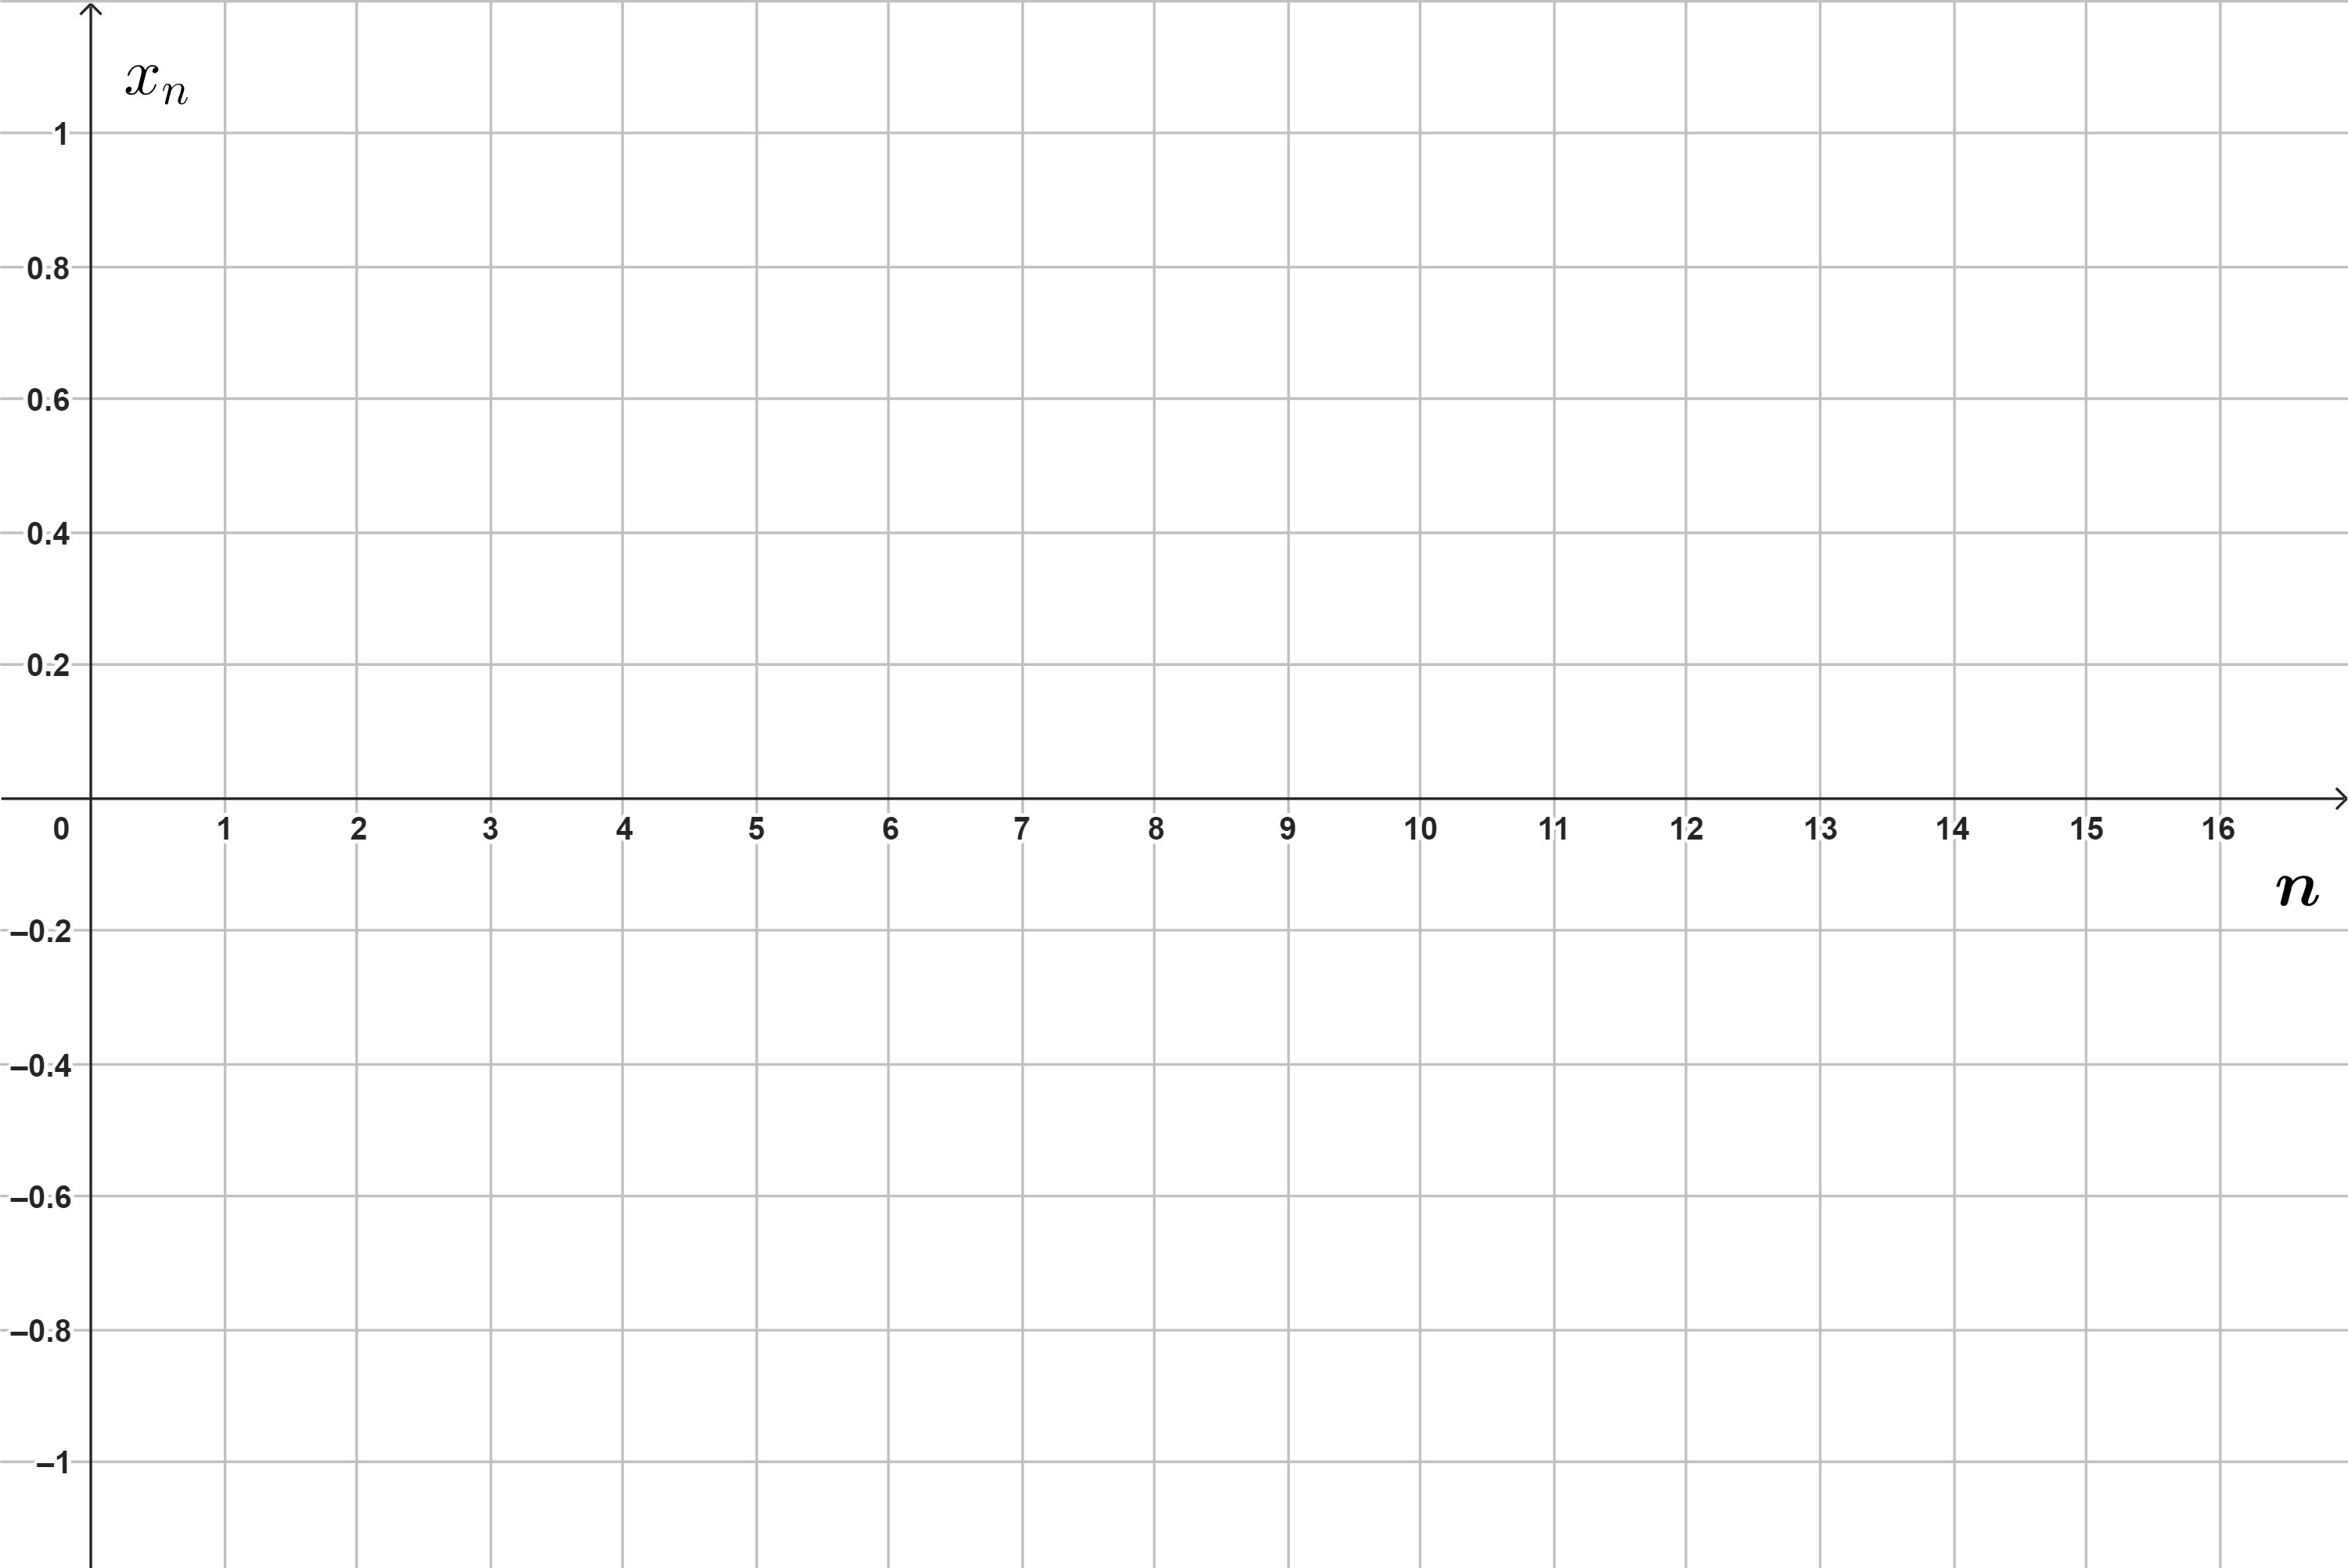
\includegraphics[scale=0.8]{Exercices/exo_sabri.png}
    \caption{Exercice \textbf{4.1 a)}}
    \label{fig:exo4.1a}
\end{figure}\\

\textbf{b)} Vers quelle limite cette suite converge-t-elle (pas besoin d'utiliser la définition à ce stade)? \\

\textbf{c)} Pour rappel, la définition de limite de suite nous dit que quelque soit l'erreur $\varepsilon$ souhaitée, aussi petite soit-elle, il existe un moment dans la suite (un naturel $N$) à partir duquel l'écart entre la suite et sa limite est inférieur à l'erreur $\varepsilon$.\\ 
Trouvez le plus petit naturel $N$ satisfaisant cette condition si on choisit comme erreur $\varepsilon = 0.1$. \\ \textbf{Indice:} Aidez-vous de votre graphique en Figure \ref{fig:exo4.1a}.\\

\textbf{d)} Généralisons la démarche du point \textbf{c)}: trouvez la condition que le naturel $N$ de la définition de limite doit satisfaire pour que l'erreur soit de $\varepsilon$.\\
\textbf{Indice:} Vous devriez obtenir une inégalité de la forme $N > f(\varepsilon)$, où $f$ est une fonction.\\

\faLightbulbO \quad \fbox{\textbf{Discutez}} Comment l'exercice change-t-il lorsque l'on considère la suite suivante?
\begin{equation}
    y_n = \frac{n^2}{n+1} \quad \forall n\in \Nn
\end{equation}

\textbf{Méthode 2: Par le théorème des suites monotones bornées}\\

\textbf{a)} Montrez que la suite \eqref{exo_suite_limite} est bornée supérieurement. Quel est son suprémum? Ce suprémum est-il un maximum (pas nécessaire pour utiliser le théorème, mais c'est bien de comprendre la distinction entre suprémum et maximum)?\\

\textbf{b)} Montrez que la suite est croissante.\\

\textbf{c)} Le théorème des fonctions monotones bornées vous permet de conclure que la suite converge (vers son suprémum, car fonction croissante dans ce cas-ci). \\ Prouvez ce théorème de manière générale pour les fonctions croissantes bornées supérieurement.\\
\textbf{Indice:} Commencez par formaliser la notion de suprémum en utilisant l'erreur $\varepsilon$ (similaire à la définition de limite: ``$\forall \varepsilon ...$''). Combinez avec la notion de croissance, puis concluez.\\

\faLightbulbO \quad \fbox{\textbf{Discutez}} Le théorème des suites monotones bornées est très pratique pour étudier la convergence de suites définies par récurrence, comme par exemple:
\begin{equation}
    x_0 = 0.5, \quad x_{n+1} = \frac{x_n + 1}{2} \quad \forall n\in \Nn
\end{equation}
Comment feriez-vous pour prouver que cette suite est bornée supérieurement(inférieurement)/\\ (dé)croissante?

\end{exercice}

\end{document}